\chapter{基于深度学习的多人姿态估计相关技术}
\label{cha:basicfacts}
本章主要围绕着基于深度学习的多人姿态估计所涉及的相关技术为主线展开论述。基于深度学习的多人姿态估计主要涉及的技术主要有三部分:基于卷积神经网络的特征提取技术、基于深度学习的目标检测方法以及基于深度学习的人体姿态估计方法,分别应用于特征提取网络的特征提取与目标检测环节(在\ref{subsec:featextract}节)与检测回归网络中(在\ref{subsec:detection}节)。
\section{基于卷积神经网络的特征提取技术}
近年来,深度卷积神经网络被普遍应用于各种视觉任务中。其中很多方法都使用在分类任务重训练好的底层网络来提取特征。同样在本文中也使用了预训练的深度神经网络为顶层网络提供特征图。因此在本小节中,本文主要介绍方法中涉及到的基于卷积神经网络的特征提取技术。
\subsection{深度卷积神经网络}
\label{subsec:factsfeature}
从2012年的AlexNet\cite{alex2012alexnet}开始兴起的深度学习和卷积神经网络热潮,让图像分类任务在准确度上获得飞跃的提升。卷积神经网络是一种深度神经网络,通过多层堆叠可学习参数的卷积核对数字图像进行卷积操作,从而在顶端,也就是网络最终层生成稠密的特征图的过程。卷积神经网络可以很好的适应数据,不仅在大型数据集的分类任务取得相当优秀的结果,还可以完成像目标检测、姿态估计等等的复杂任务。卷积神经网络可以学习数据集中不同尺度、来自不同类别物体的特征,并能够通过对这些特征的空间关系进行建模以使损失函数的输出靠近最优值。令人欣喜的是,卷积神经网络在仅给出图像标签作为训练数据的情况下,仍然可以在网络中间生成的特征中找到接近人为定义用于检测角与边的卷积核,并在更深层的网络中输出包含更多语意的特征\cite{yosinski2015understanding}。这样的特性让卷积神经网络可以获得相当强的拟合能力和泛化能力,在同样的数据集中训练会有更广的应用。同时,Mishkin等的工作中\cite{mishkin2015all}也强调使用与训练好的网络参数能够让网络得到更好的效果。因此这些在分类任务上表现良好的底层卷积神经网络结构与其参数因其优越的性能已然成为日前流行的特征提取方法。
\subsection{感受野增强的深度卷积神经网络}
\label{subsec:factsdeepextract}
抽象地说,训练深度神经网络就是在不同层级对特征的空间结构进行建模的过程。但是为了让网络尽可能学习在不同层级上特征的关联,就必须从结构上扩大卷积层能够影响的区域。为了达成这一目标,通常会借助能够描述网络顶层卷积核的有效作用区域的指标,也就是感受野,来帮助设计具有合适深度的网络。在考虑感受野大小的前提下设计网络,首先不会设计远远超出需求的网络结构,导致更多的计算与更困难的训练,同时也不会因为感受野不足而导致性能下降。

正如Luo等工作\cite{luo2016understanding}中提出的,感受野区域大小对于卷积神经网络非常重要。能够让网络获得获得更大感受野的方式主要有三种方式:使用池化层减少特征图的分辨率;堆叠卷积层;调整卷积步长或卷积策略。为了方便理解,感受野可以被可视化为图\ref{fig:ReceptionField}。图\ref{fig:ReceptionField}左侧将每个像素的作用区域映射到底层原图(蓝色)上(灰色)。右侧将顶层得到的特征图转换成稀疏的形式,每层卷积核的感受野分别以绿色与黄色标记在图中。在这里可以很直观地理解,如果网络没有足够的感受野大小,比如一个超出图\ref{fig:ReceptionField}中右侧中黄色区域大小的物体,那么此时得到的仅仅是不超过黄色区域几个邻近区域的特征响应,而不是能够考虑到物体整体的结果。这样会影响神经网络的性能,尤其是对于一些对精度要求很高的网络,比如用于目标检测任务或关键点检测任务的神经网络。

\begin{figure*}[htbp]	
	\centering
	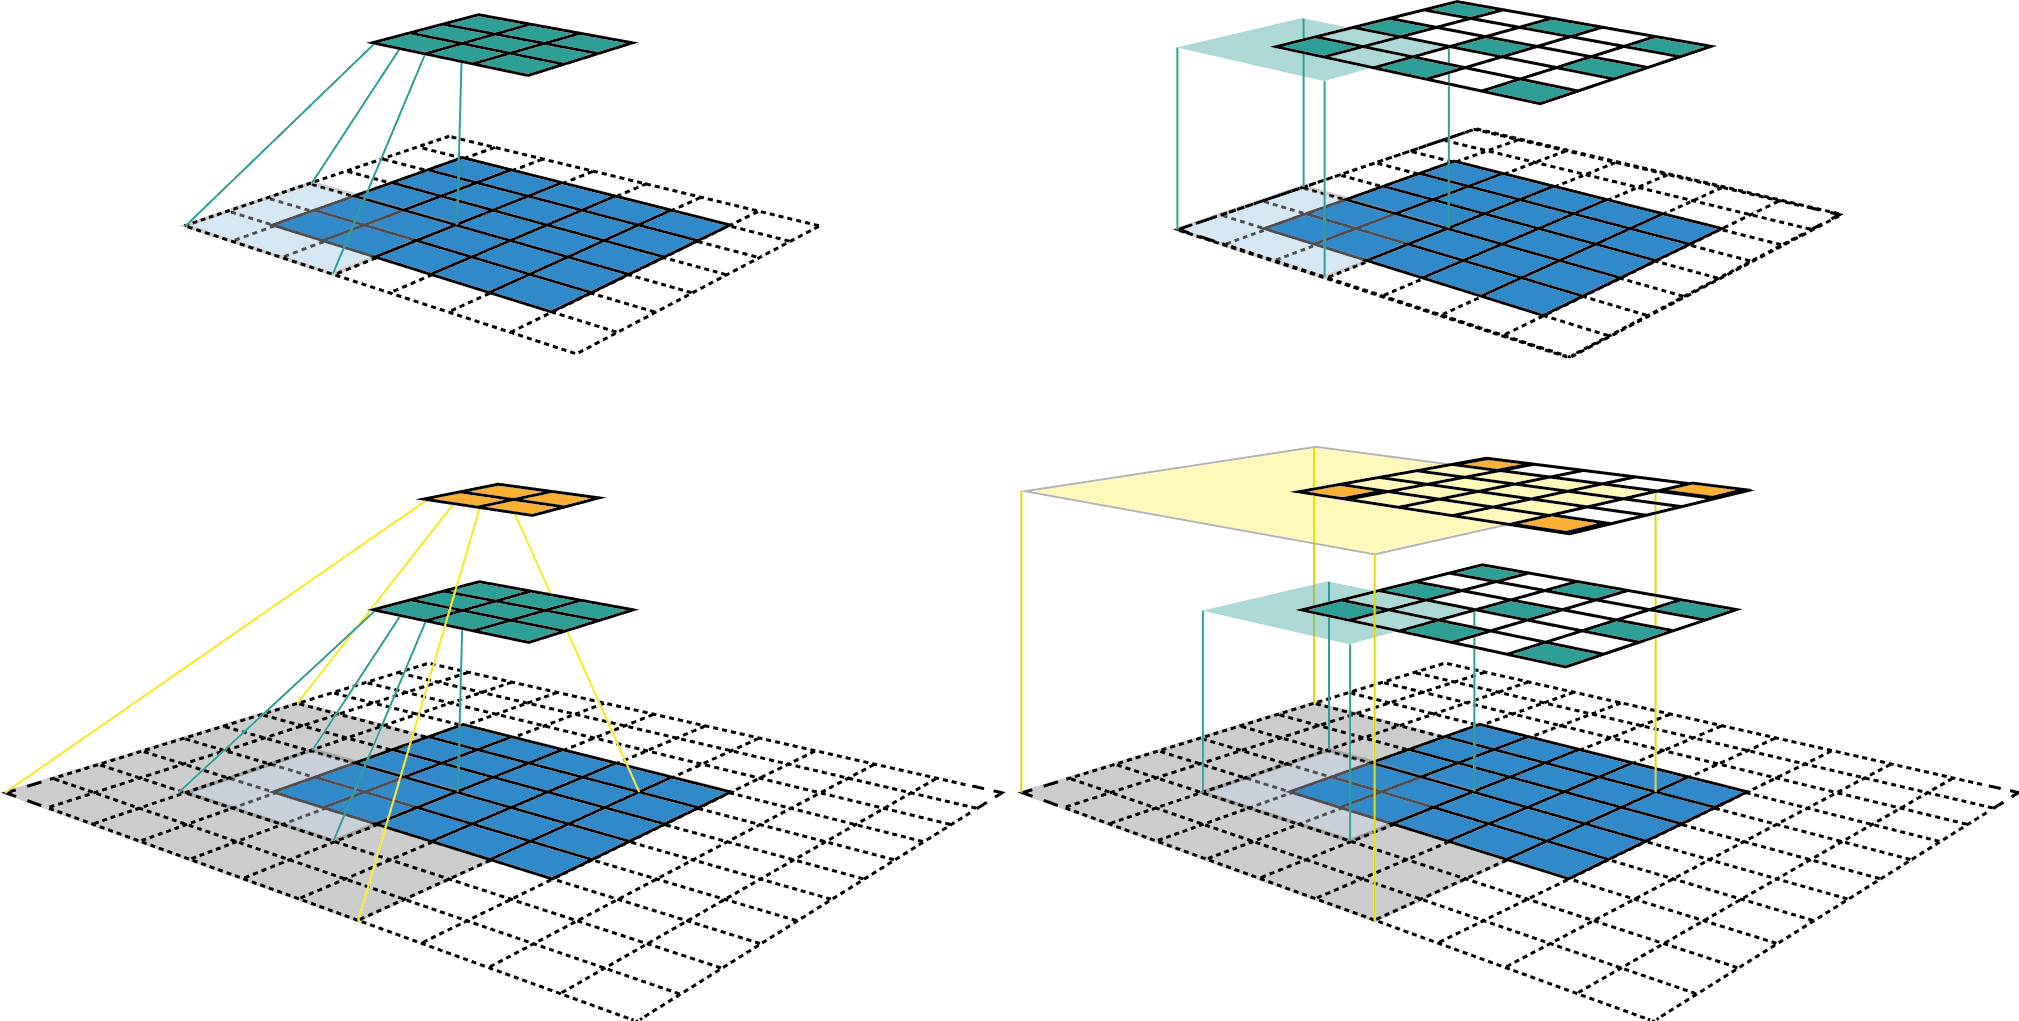
\includegraphics[width=0.8\textwidth]{ReceptionField.png}
	\caption{两种可视化感受野的方法\cite{fang2017reception}}
	\begin{minipage}{0.8\textwidth}
		\wuhao
		注:左侧两幅图分别为单层和多层的感受野大小可视化结果,其中灰色的部分是有效感受野的方法。与左侧图示不同的是,右侧图示中将深层卷积得到的稠密特征图按照输入尺寸进行稀疏化处理,就可以将有效感受野区域重新映射回结果特征图上,就如右侧图中绿色与黄色区域所示。
	\end{minipage}
	\label{fig:ReceptionField}
\end{figure*}

%	Good performance in Classification -> better performance
之所以认为神经网络具有很强的特征提取能力,是因为将在图像分类任务中训练得到的网络参数迁移到解决其他图像任务的网络模型中可以更好地引导网络得到更好的结果\cite{mishkin2015all}。同时根据Yosinski等人的工作\cite{yosinski2015understanding},在可视化结果中,的确可以看到在分类标签监督下的网络参数对具有语意的区域有较强的响应。所以,大部分希望提高网络特征提取能力的方法都会把目光聚焦在图像分类这一视觉基础任务上。因为在分类任务上更好的性能就意味着网络在特征提取上更强的鲁棒性。

He等人在2015年提出残差网络\footnote{残差网络,Residual Network,通常被称为ResNet。并且根据具体的层数来分别称呼同种方法的不同的结构,例如101层的残差网络,会被称作ResNet-101。}结构\cite{He2015Deep}。如图\ref{fig:Resblock},文章设计了带有跳跃连接残差模块,将梯度跨层传入浅层的网络,改善在试图构建深度网络时出现的收敛问题,比如在使用类似VGG网络\cite{simonyan2014very}的策略扩大网络深度时遇到的梯度消失问题。同时,为了减少极大值池化层带来的特征损失,残差网络在下降特征图尺寸时使用了步长为2的卷积层。通过堆叠普通残差模块或瓶颈残差模块,网络能够获得比之前简单堆叠卷积层的策略更加好的分类准确度,和更加稳定的收敛结果。

\begin{figure*}[htbp]	
	\centering
	\begin{subfigure}[b]{0.35\textwidth}
		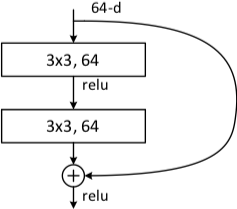
\includegraphics[width=\linewidth]{ResBlock_a.png}
		\caption{普通残差模块}
	\end{subfigure}
	\hskip1.5cm
	\begin{subfigure}[b]{0.35\textwidth}
		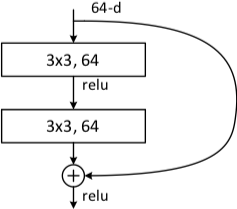
\includegraphics[width=\linewidth]{ResBlock_a.png}
		\caption{瓶颈残差模块}
	\end{subfigure}
	\caption{残差模块结构\cite{He2015Deep}}
	\label{fig:Resblock}
\end{figure*}
\begin{figure*}[htbp]	
	\centering
	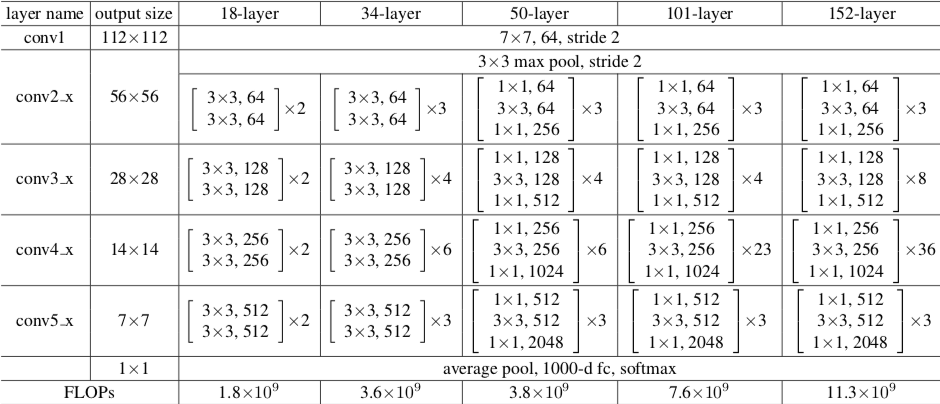
\includegraphics[width=0.8\textwidth]{ResNet.png}
	\caption{残差网络结构\cite{He2015Deep}}
	\label{fig:ResNet}
\end{figure*}

在残差网络初始的结构策略中,残差薄块可以最多堆叠至152层,如图\ref{fig:ResNet}所示。残差模块的出现让更深层次的网络成为了可能,甚至于在竞赛中出现了千层以上的残差网络。利用残差模块构建深层卷积神经网络来提取特征已经成为了现在使用卷积神经网络的方法普遍做法。残差网络易收敛,大感受野的良好特性让其在各种任务重都能够起到相当重要的作用。

\section{基于深度学习的目标检测技术}
\label{sec:factsobjectdetection}
目标检测对于自顶向下的多人姿态提取而言是十分重要的。由于本文中也使用了一些基于深度学习的目标检测技术,因此在本节简短介绍一下目标检测的相关技术。

\subsection{锚点与检测框}
\label{subsec:factsanchors}
目标检测任务的前身是目标定位,对给定的一个物体进行边界框回归\cite{ILSVRC15}。在一些使用卷积网络的目标定位方法中,坐标由四个独立的全连接神经元回归而成,如图\ref{fig:SingleBox}所示。虽然这种方式的确能够回归单个检测框,然而却不能回归出多个检测框。

在DeepMultiBox中使用的坐标回归\cite{erhan2014scalable}将多个边界框的四个坐标串联成了一个向量,并对向量进行回归。这种方法只能生成有限数目的边界框。同时,使用全连接层作为回归所有边界框的分支需要较为复杂的匹配规则来让全连接输出与位置对齐。实际上,卷积网络反而更加适合用于回归粗略的边界框。假定我们有几组给定大小,给定长宽比的默认边界框,如果能够回归得到这些默认边界框的中心,那么就可以得到完整的检测结果。因此,锚点的概念就油然而生。

为了让网络能够在一张图中检测到多个检测框,1\times1卷积层替换掉了传统的全连接层,用来回归分类结果、横纵坐标的偏移量与长宽尺寸的偏移量,如图\ref{fig:MultiBox}所示。与单检测框方法直接回归坐标不同,多检测框方法中的输出张量中每一个像素位置代表一个检测框,因此这些像素位置本身就包含着类别标签、坐标与尺寸信息。这些像素位置都被称作锚点,使用类别标签来确定候选框的位置,之后经过回归的对应像素位置上的坐标与尺寸偏移量会与锚点所属的坐标与尺寸结合,得到最后的检测框。这种使用卷积回归锚点来得到检测框的方法,已经广泛被应用在了单阶段和两阶段的目标检测网络中,比如YOLO\cite{redmon2016you}和Faster R-CNN\cite{Ren2015Faster}。

\begin{figure}[h]	
	\centering
	\begin{subfigure}[b]{0.4\textwidth}
		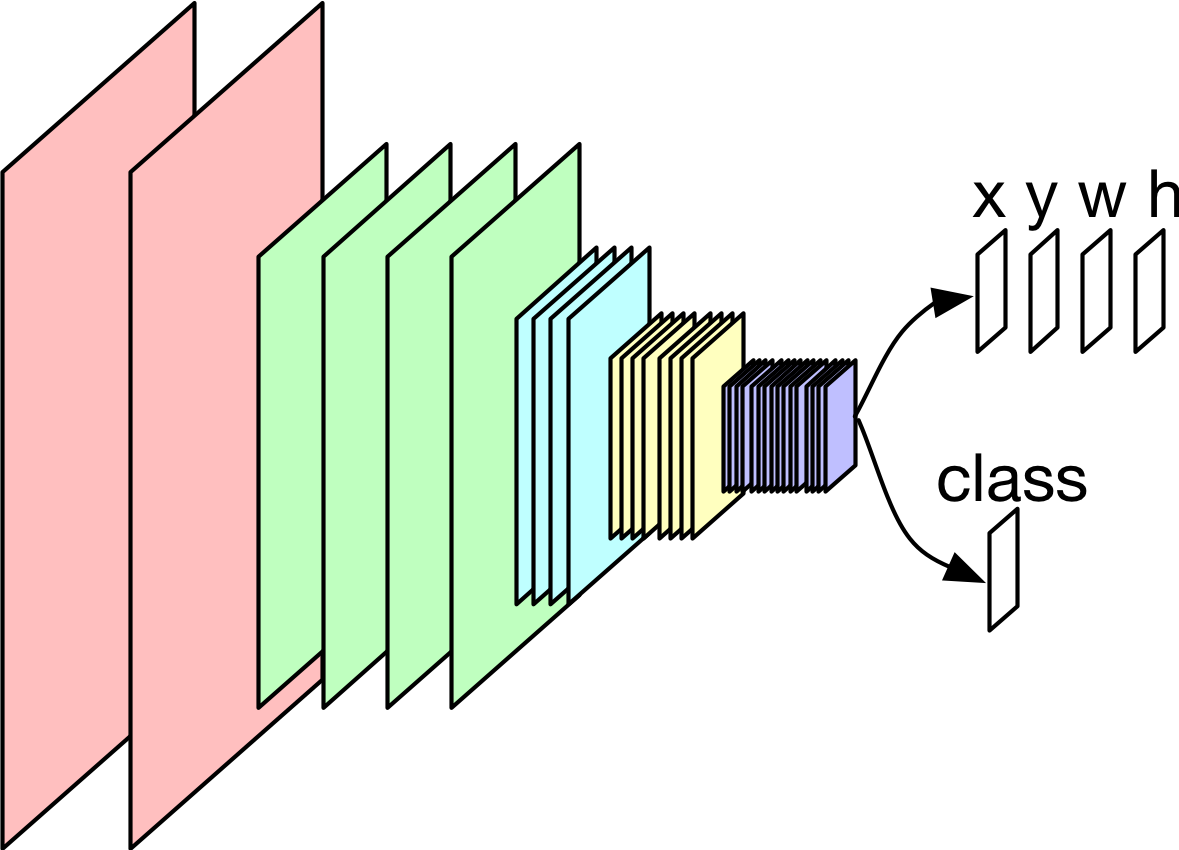
\includegraphics[width=\linewidth]{SingleBox.png}
		\caption{用于定位的单检测框方法}
		\label{fig:SingleBox}
	\end{subfigure}
	\hskip1.5cm
	\begin{subfigure}[b]{0.4\textwidth}
		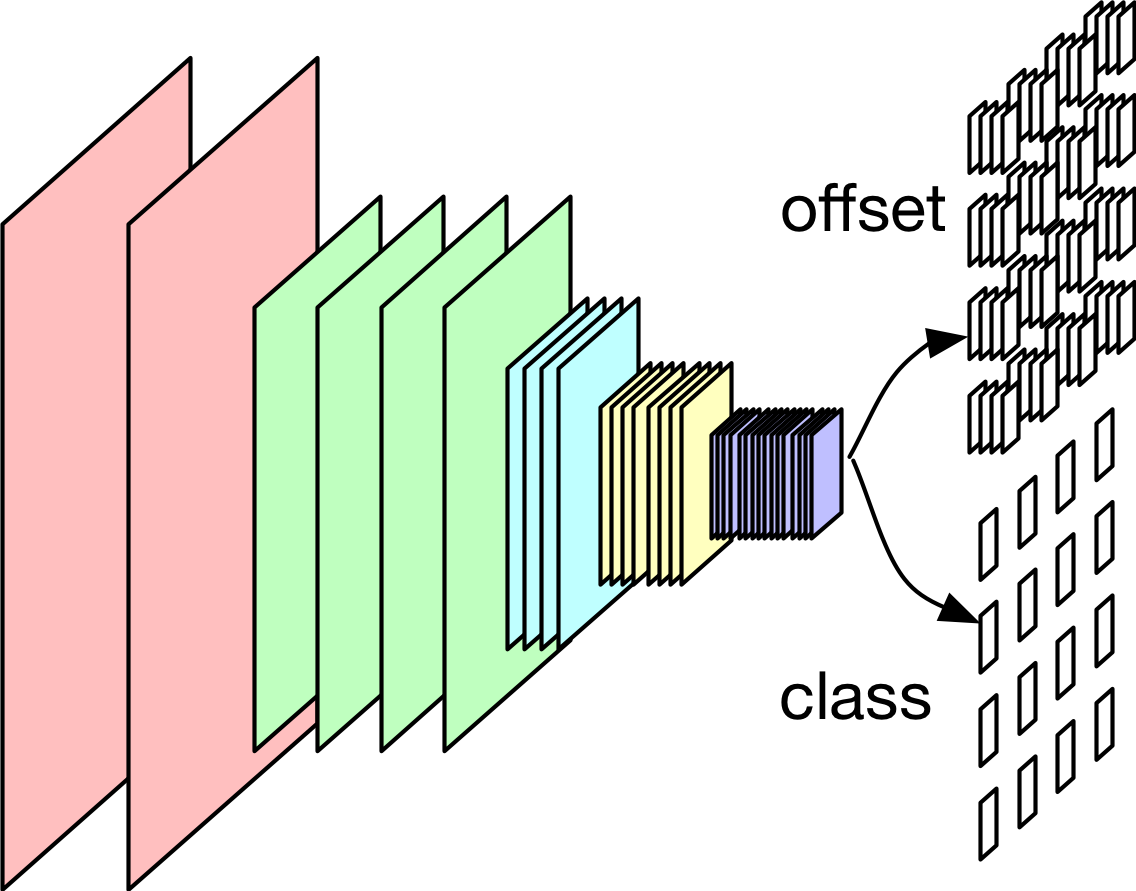
\includegraphics[width=\linewidth]{MultiBox.png}
		\caption{用于检测的多检测框方法}
		\label{fig:MultiBox}
	\end{subfigure}
	\caption{基于卷积神经网络的定位与检测方法}
\end{figure}

\subsection{区域建议网络与回归网络}
\label{subsec:factsRPNregression}
目标检测任务不光要求算法给出检测框结果,同时要给出分类结果。对于每一个检测框算法都需要给出一个类别标签。为了继续保持如图\ref{fig:SingleBox}中的单检测框方法的结构,一些方法,比如Faster R-CNN\cite{Ren2015Faster},将网络分为两个阶段:在第一阶段中,使用类似图\ref{fig:MultiBox}的结构,在文章中被称作区域建议网络\footnote{区域建议网络,Region Proposal Network},仅对物体进行前背景分类,并且使用较为贪婪的策略寻找可能是物体的检测框;第二阶段中,网络使用类似图\ref{fig:SingleBox}所示的结构,将裁剪后的特征送入全连接层对物体分类并对偏移量进行第二次回归。但值得一提的是,一些单阶段的检测器,就是仅使用图\ref{fig:MultiBox}结构的检测器也可以给出较为精确的结果。不过由于漏检率稍高,单阶段检测器从性能上并不能完全压制两阶段的检测方法。

\section{基于深度学习的多人姿态估计技术}
\label{sec:factspose}
相比目标检测,多人姿态估计的方法更加要求精度。同时,为了考量人体姿态中结构化的信息,网络还需要更多的感受野来对姿态结构进行学习。因此如何以张量形式定义关键点信息与如何监督深度网络成为了姿态估计方法中的两个非常重要的技术。

\subsection{关键点与热图}
\label{subsec:factsheatmaps}
关键点信息与一般的坐标回归不同,其响应对应的区域更小。目标检测中一个锚点对应的是一个物体,也就是至少十余像素边长的范围。但在关键点则不同,一个关键点对应的躯干部位至多几像素大小。对于这样小的区域,如果使用目标检测中的回归锚点位置与偏移量的方法进行学习,是很难让让网络给出鲁棒的响应的。因此常见的关键点表示方法一般是使用多张热图组成的张量共同描述不同关键点的位置。如图\ref{fig:keypointhm}所示,张量中每一通道的热图都表示一类关键点出现的概率,其中单张热图中预测概率的极高值就是网络最终输出的结果。在自顶向上的方法中,一般仅取热图中的最大值作为结果,然而对于自底向下则需要提取更多的关键点。并且在提取更多关键点的时候,要使用极大值抑制来限制过近的位置对其他区域极值点的竞争。

\begin{figure}[h]	
	\centering
	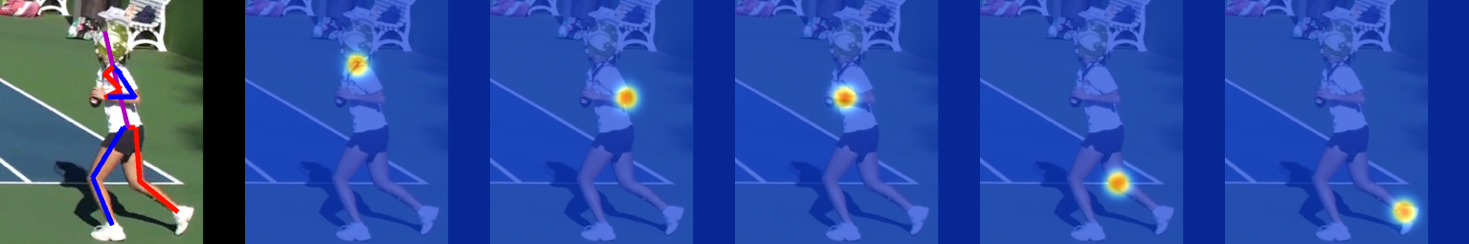
\includegraphics[width=\textwidth]{keypointhm.png}
	\caption{人体关键点热图的每个通道包含对骨架中的每一个关键点的位置估计\cite{newell2016stacked}}
	\label{fig:keypointhm}
\end{figure}

这里有一个很明显的问题:关键点热图的分辨率可能影响最终姿态估计精度。那么为了解决这一点,多数方法故意不使用使用二值响应或标签作为训练数据,而是使用了高斯分布来描述关键点的位置信息。这意味着,在这种监督下,网络在这样的标注数据下将倾向于在关键点的周围生成一些环境响应。这些环境响应并不是没有作用,而是在后处理中,被用于帮助算法通过双线性差值的方式寻找重新映射为真值尺度下的关键点坐标。这样能够较为较为有效地改善低分辨率热图影响姿态估计网络精度的问题。

\subsection{中继监督}
\label{subsec:factsintersupervision}
由于姿态估计算法需要完整考虑人体关键点之间的结构,同时对结果的精度要求也很高,所以相比其他任务而言对感受野大小的要求更为严格。在设计姿态估计网络时,许多工作都是通过增加网络深度的方式来扩大感受野。在监督过深的神经网络时,正如\ref{subsec:factsdeepextract}节中所描述时,会遇到梯度消失的问题而导致过深的网络在性能上出现退化的现象。在Wei等人的工作中\cite{wei2016convolutional}首次提出了中继监督的技巧。中继监督主要是通过将网络切分成完全一致的多个阶段,在每阶段的顶端都加入相同的监督信息约束网络生成相似的结果。同样在堆叠沙漏网络(SHN, Stacked Hourglass Network)\cite{newell2016stacked}中也同样使用了残差的方式分阶段进行中继监督。这样的技巧主要是旨在解决过深网络中出现的梯度消失问题。中继监督的确能够很好地解决多人姿态中出现的收敛问题,因此这一技术已经成为了现有姿态估计方法中定会采用的监督策略。

\section{本章小结}
本章简略介绍了基于深度卷积神经网络的多人姿态估计所涉及的技术。首先,本章由对基于卷积神经网络的特征提取技术简介开始,说明了特征提取器以及感受野对于网络设计的影响。对感受野的所用分析可以引出本文对网络模块设计的基本原则。紧接着本章通过对比单检测框与多检测框的检测方法解释了锚点在目标检测的重要性。这部分能够帮助理解在特征提取网络中检测目标框的技术细节。最后,本章通过阐述关键点回归与边界框回归任务的不同解释了热图在关键点回归中的必要性,同时简略介绍了中继监督的目的与方法。这部分简介可以帮助理解中继监督在姿态估计网络训练中的意义。
